% Wirtschaftliche Machbarkeit

\section{Wirtschaftliche Machbarkeit} \label{section:wirtschaftlichemachbarkeit}

\subsection{Aufwandsabsch�tzung}

\begin{figure}[h]
	\centering
		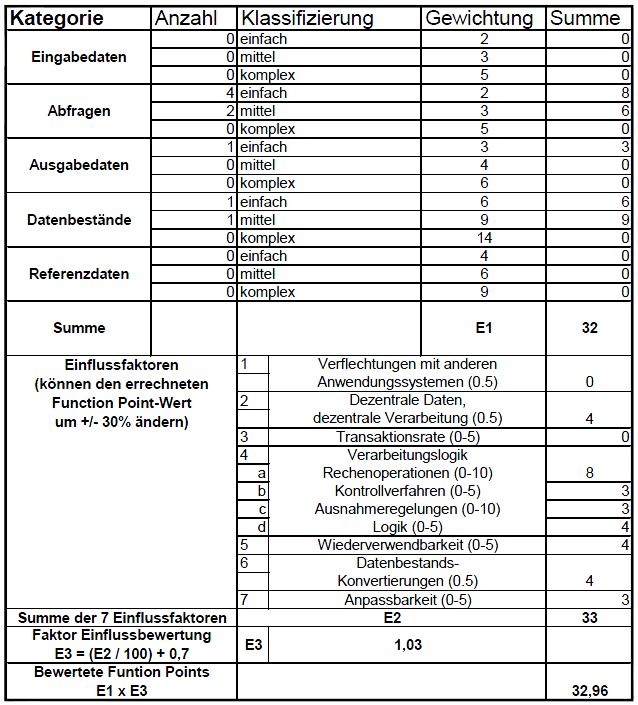
\includegraphics{graphics/wirmachbarkeit/FunctionPointsAnalysis.JPG}
	\label{fig:FunctionPointsAnalysis}
\end{figure}

\subsection{Nutzen}

\subsection{Pr�fen der Risiken}
\subsubsection{Personenausfall}
Eintrittswahrscheinlichkeit:  gering \\
Auswirkungen:  								hoch   \\

In dem unerwarteten Fall, dass ein Teammitglied l�ngerfristig ausf�llt, muss es m�glich sein die Arbeitsaufgaben dementsprechend neu aufteilen zu k�nnen.
Folgende F�lle k�nnten auftreten:
\begin{itemize}
	\item Streit im Team
	\item Ausfall durch Krankheit oder Tod eines Teammitglieds
	\item Austritt eines Teammitglieds aus dem Projekt
	\item Der Auftraggeber k�nnte aufgrund von Unklarheiten den Projektabbruch initiieren 
	\item Es kann passieren, dass von Seite des Auftragsgebers pl�tzlich kein Interesse an der Umsetzung des Produktes mehr gegeben ist, und es dadurch zu extremem Zeitverzug kommt, was bis zum Abbruch f�hren kann
	\item Interessensverlusst eines Teammitglieds, und damit verbundene minderwertigere Arbeit 
\end{itemize}

Folgende pr�ventive Ma�nahmen werden eingef�hrt:
\begin{itemize}
	\item Regeln f�r den Umgang innerhalb des Projekts
	\item Ausreichendes Interesse jedes Mitglieds und keine leistungstechnische Probleme 
	\item Gutes Verh�ltnis mit den Auftraggebern
\end{itemize}

\subsubsection{Zeitliche Risiken}

Eintrittswahrscheinlichkeit:  gering \\
Auswirkungen:  								mittel \\

Die Aufwands- und Zeitsch�tzung basiert auf dem derzeitigen Lastenheft des Auftraggebers und stellt eine zeitgerechte Fertigstellung sicher. Sollten sich jedoch die Anforderungen des Kunden w�hrend des Projekts �ndern, so wird sich das mit gro�er Wahrscheinlichkeit verz�gernd auf den Fertigstellungstermin auswirken. Die mit dem Kunden vereinbarte Funktionsanalyse und die Meilensteine mit gemeinsam festgelegten Qualit�tskriterien sollten jedoch diesem Risiko entgegenwirken.

\subsubsection{Technische Risiken}
\label{subsection:Technische Risiken}
\textbf{Datenverlust}\\
Eintrittswahrscheinlichkeit:  gering \\
Auswirkungen:  								mittel \\

Aufgrund der nicht auszuschlie�enden Gefahr des Datenverlusts, muss daf�r gesorgt werden die Sicherheit der Daten, sowie auch die Verf�gbarkeit dieser zu garantieren. Dieses Problem wird mithilfe eines \gls{git} gel�st, durch diesen Server ist es m�glich die Versionen der Software immer zug�nglich zu machen und zus�tzlich die Daten auf den Computern der Projektmitgliedern zu speichern. \\ \\

\textbf{Hardwareausfall} \\
Eintrittswahrscheinlichkeit: gering \\
Auswirkung: mittel \\

Es kann ohne jede Vorwarnung immer und �berall ein Hardwareausfall passieren, dies kann selbst verschuldet, aber auch pl�tzlich passieren. Um mit einem solchen Ausfall zurecht zu kommen besitzt das Projektteam einen Ersatzlaptop um das gezielte Arbeiten auch nach dem 
Ausfall garantieren zu k�nnen. \\ \\

\textbf{Versionsverlust} \\
Eintrittswahrscheinlichkeit: sehr gering \\
Auswirkung: mittel \\

Bei den Versuchen mit dem Algorithmus wird andauernd etwas in der Datei ver�ndert. Bei dieser T�tigkeit kann es passieren das die Zusammenh�nge zwischen 1 oder mehreren Versionen des Algorithmus verloren gehen. Bei so einem Verlust kann auch das grundliegende Verst�ndnis f�r die jeweilige Version verloren gehen.\\
Folgende pr�ventive Ma�nahmen werden eingef�hrt:
\begin{itemize}
	\item Verwendung eines \gls{git}, f�r die automatische Versionierung
	\item Zwingende Benutzung der Bugtrackingsoftware
	\item Kommunikation im Team �ber die �nderungen am Algorithmus
\end{itemize}